
\noindent
Integrating curvilinear geometries into modelling software is not an easy task. It requires meshing software capable of creating accurate higher order elements from analytic designs or experimental data, curvilinear grid manager able to efficiently manipulate such elements (e.g. perform coordinate mapping and integration), as well as a PDE solver able to exploit the curved geometries. Ideas of using curvilinear grids first appeared in the literature in the 1970s \citep{ciarlet+1972, lenoir1986} and have been used in electromagnetic simulations for at least two decades \citep{wang+1993}. 

%%
\noindent
A impressive example of using a curvilinear $3$-dimensional code together with DG and optimized for parallel GPU processing can be found in the aerodynamics community \citep{Warburton2012}.
%%
\citeauthor{wang+2011}\citep{wang+2011} demonstrate a 3D curvilinear parallel DG code for solving Maxwell's equations in a homogeneous medium.
%%
Still, they are much less widespread than linear meshes and so far have only been explicitly presented in 2D codes \citep{wang+2011a}.
%%
Having finished the implementation of a curvilinear code ourselves, we believe that the challenges causing this lack of adoption are as follows:
\begin{itemize}
\item Generation of curvilinear meshes is a challenging process, as naive approaches can easily result in self-intersecting meshes \citep{toulorge+2013, johnen+2012};
\item Standard functionality of a grid manager, such as interpolation, local-to-global and global-to-local mappings, integration, calculation of normals and basis functions becomes significantly more difficult; additional numerical tools, such as Lagrange interpolation, adaptive integration, analytical polynomials, and optimization algorithms have to be employed to provide the desired functionality
\item Ensuring that the geometry accurately describes the material boundary is insufficient to achieve convergence of the desired polynomial order. The curvature of the interior has to be taken care of as well \cite{lenoir1986}.
\item In order to fully benefit from the curved geometries through reducing the total element count, basis functions of order sufficient to resolve the detailed structure of the field are necessary. \citeauthor{fahs2011}\citep{fahs2011} implements a serial time-domain 2D and 3D curvilinear DG code and studies the scaling of the accuracy of electromagnetic benchmarks (\textit{Mie} scattering and layered \textit{Mie} scattering) depending on p-refinement. He finds that only in curvilinear geometries increasing the basis function order significantly improves the solution accuracy.
\end{itemize}

\noindent
To the best of our knowledge, the combination of higher order curvilinear meshes and domain decomposition has not yet appeared in a parallel DGFD code. Until recently, literature presents implementations of such codes with several simplifications, limiting the the flexibility and detail achievable on moderate computational resources. \\

\noindent
Nevertheless, higher order geometries carry large potential. The fundamental target is to improve the accuracy of the solution given a fixed computational resource, and curvilinear geometries can offer that. The curvilinear material boundaries have smooth corners unlike their linear analogues \cref{fig:result:spherecurv}, avoiding the unphysical local field enhancement, or the need to go to very small element sizes. \\

\begin{figure}
    \centering
	\begin{subfigure}[b]{0.48\textwidth} \hspace{8mm} 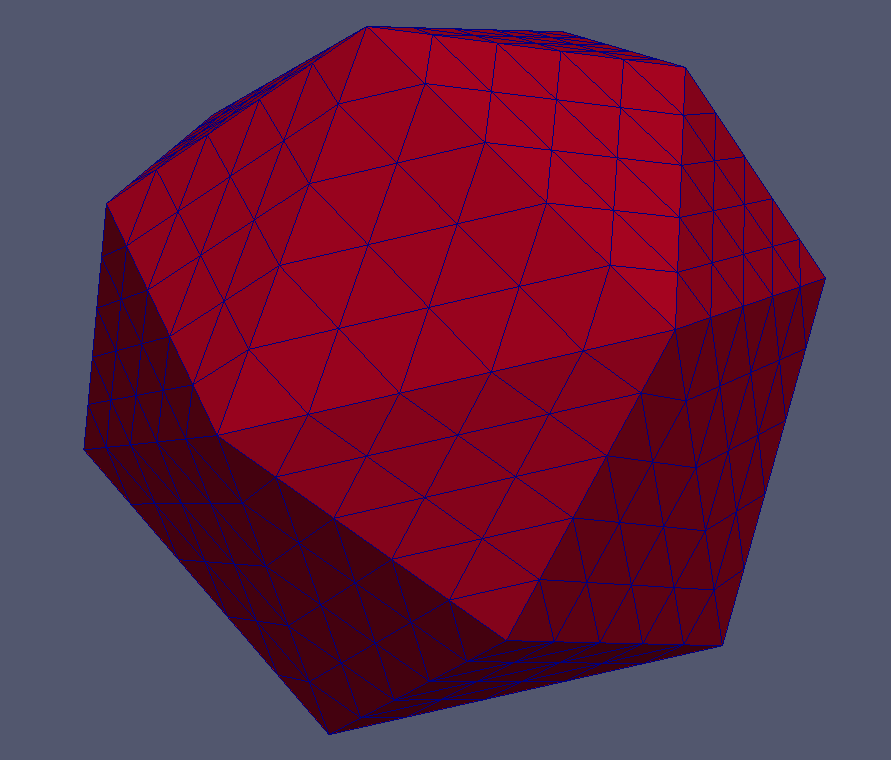
\includegraphics[scale=0.215]{images/sphere32discr6ord1} \end{subfigure}
	\begin{subfigure}[b]{0.48\textwidth} 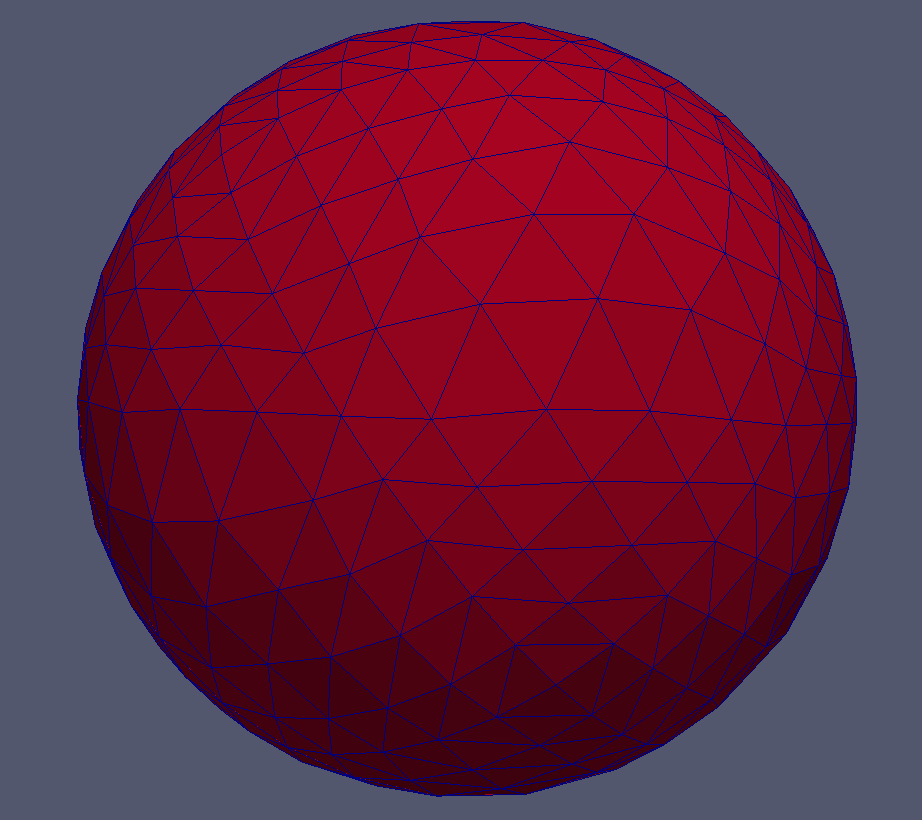
\includegraphics[scale=0.2]{images/sphere32discr6ord5} \end{subfigure}
	\captionsetup{width=0.8\textwidth} 
	\caption{Presented is the 32 Tetrahedron mesh of a sphere, using first and fifth order polynomial interpolation. Visualisation software does not easily support curvilinear elements, so the elements are discretized by CurvilinearVTKWriter by a set of smaller linear tetrahedra to visualise curvature }
	\label{fig:result:spherecurv}
\end{figure}

\noindent
Further, the accuracy of the solution improves much faster when increasing the order of basis function inside each element (increasing basis function order), as opposed to increasing the number of basis functions \cite{jin2014} \cref{fig:jin:basisconv}. However, in case of smooth material boundaries this effect can only be exploited if the corresponding element geometries are of sufficiently high order \cite{fahs2011} \cref{fig:fahs:curvconv}. Finally, while the curvature of the material surfaces is clearly defined by those surfaces, to actually achieve higher order convergence of the solution, extra care needs to be taken when choosing the seemingly-arbitrary curvature of surfaces and volumes inside the homogeneous material \cite{lenoir1986}.

\begin{figure}
    \centering
    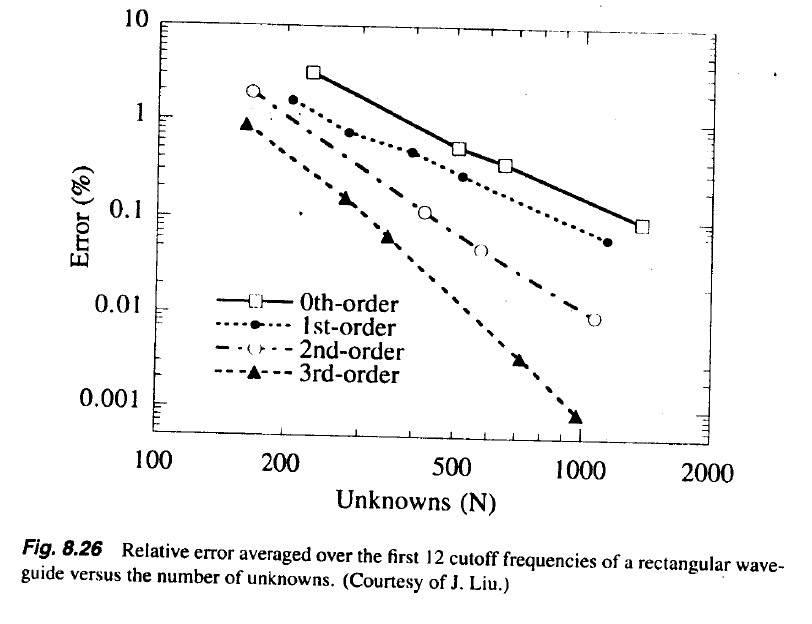
\includegraphics[scale=0.4]{images/Jin-basis-function-efficiency}
	\captionsetup{width=0.8\textwidth} 
	\caption{ \citeauthor{jin2014} shows that using the same resource, the accuracy improves faster by increasing the basis function order, than by refining the computational mesh }
	\label{fig:jin:basisconv}
\end{figure}

\begin{figure}
    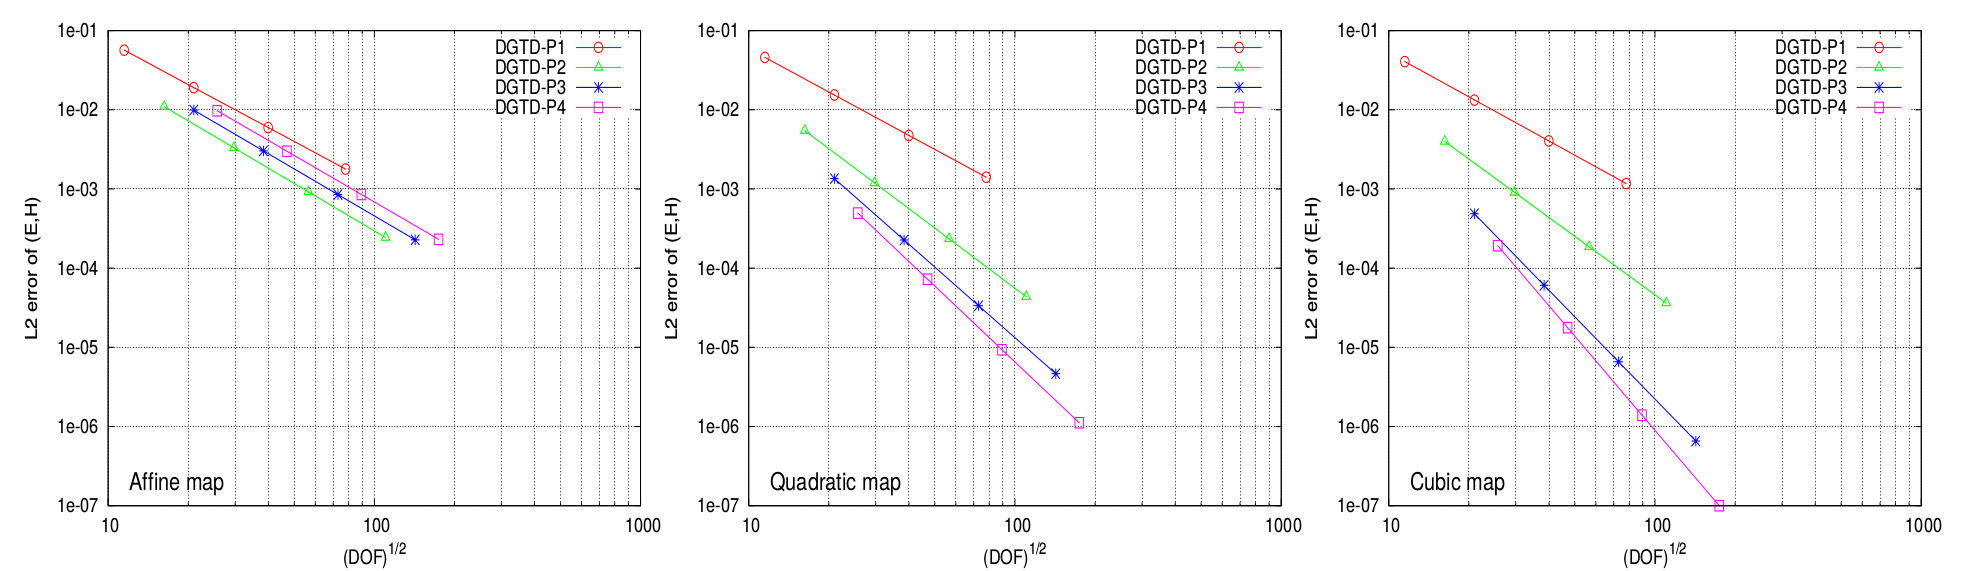
\includegraphics[scale=0.25]{images/fahs-convergence}
	\captionsetup{width=0.8\textwidth} 
	\caption{ \citeauthor{fahs2011} shows that computational accuracy (in terms of $L_2$ error) improves with increasing basis function order, but it improves faster if the element interpolation order increases as well   }
	\label{fig:fahs:curvconv}
\end{figure}


\subsection{Capabilities of CurvilinearGrid}
\label{section-outline-capabilities}

The Curvilinear Grid (CurvGrid) is a self-consistent grid manager supporting 3D tetrahedral curvilinear grids. It depends on the core modules of Dune \citeDune{}, as well as an external parallel mesh partition library Parmetis \citeParMetis{}. Also, the CurvGrid depends on Curvilinear Geometry (CurvGeom), also developed by us as a separate dune-module. \\

\noindent
CurvGeom is capable of managing curvilinear simplex elements of orders 1-5 via hard-coded Lagrange Polynomials. It also has the capability to manage arbitrary order simplex geometries via analytic Largange Interpolation method. CurvGeom complies with standard dune-geometry interface, providing methods for local-to-global and global-to-local coordinate conversion, computation of Jacobian matrix, integration element and volume. There is also a cached version of CurvGeom which pre-computes the local-to-global map and its determinant, and is thus considerably faster than its non-cached analogue. Additionally, CurvGeom provides the methods to obtain outer normals of subentities of this geometry, and the subentity geometries themselves. Also, CurvGeom implements a polynomial class and associated differential methods, which allow to obtain analytical expressions for local-to-global map and associated integration element, enabling exact manipulation of geometries of arbitrary order. Finally, CurvGeom contains its own recursive integration tool (based on quadrature provided by dune-geometry) for integrating non-polynomial integrands. The reason for implementing this functionality is due to integration elements being non-polynomial in general case (see \cref{sec:theory:integration}). For example, the face area of a curvilinear element is given as an integral over a square root of a polynomial. \\

\noindent
CurvGrid is supplied with its own Curvilinear GMSH Reader (CurvReader). CurvReader is designed to read curvilinear \textit{.msh} files of orders 1 to 5, where 1 corresponds to linear meshes. CurvReader is parallel-scalable meaning that each process only reads the necessary part of the mesh, avoiding memory overflow. CurvReader has the option to partition the mesh using ParMetis during the reading procedure, further decreasing the file access time. CurvReader also reads physical tags provided GMSH and supplies the Grid Factory with this information. \\

\noindent
Curvgrid is also supplied with its own Curvilinear VTK Writer (CurvWriter) to output the grid into VTK, VTU or PVTU file formats. CurvWriter will write either the entire grid, or the set of elements supplied by user. It provides each element with data about its rank, partition type and physical tag, which can be used to visually inspect the parallel connectivity of the domain \cref{fig:result:spherestruct}. We have tested the scalability of the grid assembly and visualisation on a single 12 core machine using a 4.4 million element tetrahedral mesh \cref{fig:result:bullseye}. The mesh can be supplied with arbitrary number of vector fields to visualise, e.g. the solution(s) of a PDE. We have tested the visualisation of CurvGrid using ParaView \cite{johnson+2005} and VisIt \cite{childs+2012} end user software. \\

\begin{figure}
	\begin{subfigure}[b]{0.30\textwidth} \hspace{4mm} 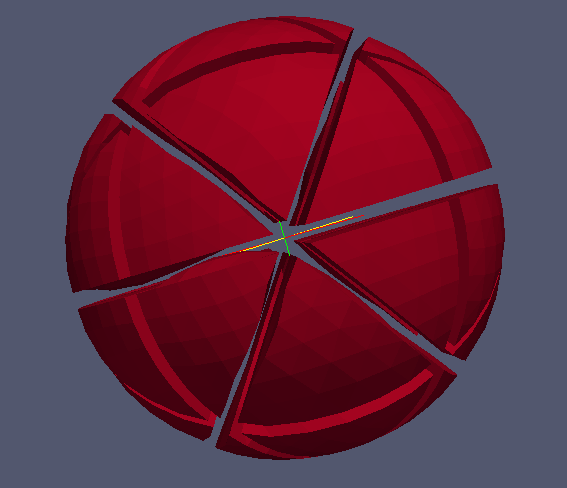
\includegraphics[scale=0.22]{images/32-inter} \captionsetup{width=0.8\textwidth} \caption{ Interior elements used to discretize the field} \end{subfigure}
	\begin{subfigure}[b]{0.30\textwidth} \hspace{4mm} 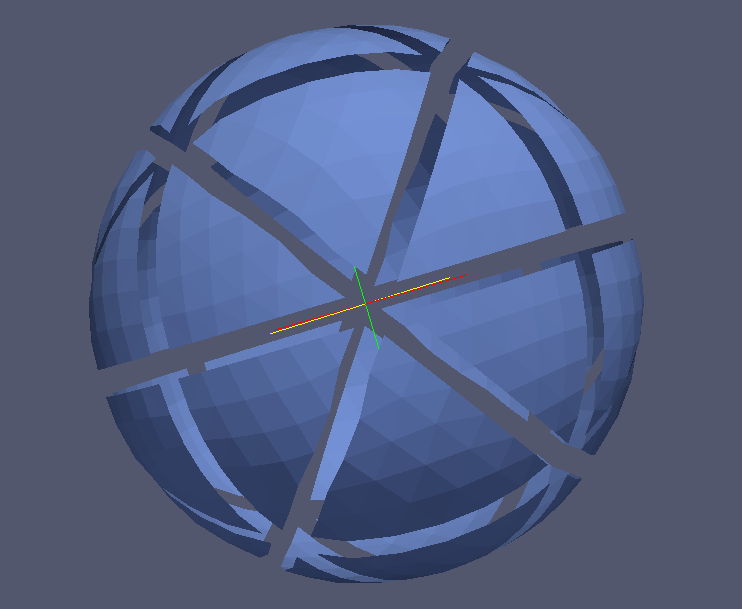
\includegraphics[scale=0.18]{images/32-db}    \captionsetup{width=0.8\textwidth} \caption{ Domain boundaries used to discretize the boundary condition} \end{subfigure}
	\begin{subfigure}[b]{0.33\textwidth} \hspace{4mm} 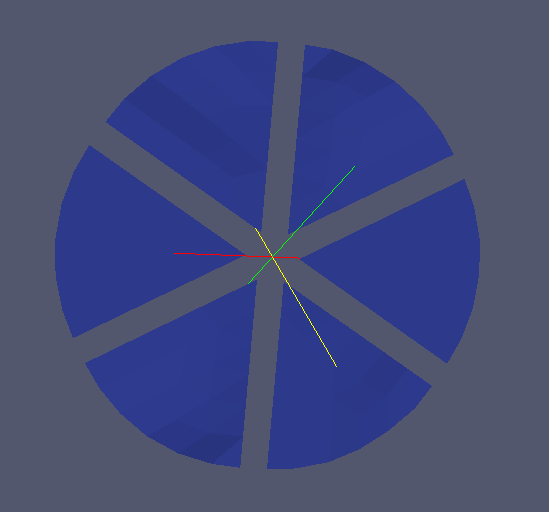
\includegraphics[scale=0.22]{images/32-pb}    \captionsetup{width=0.8\textwidth} \caption{ Process boundaries used to communicate between neighbouring processes} \end{subfigure}
	\begin{subfigure}[b]{0.46\textwidth} \vspace{5mm} \hspace{12mm} 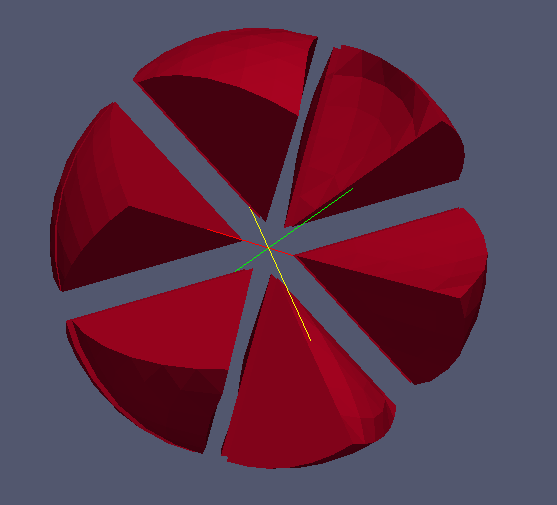
\includegraphics[scale=0.25]{images/32-ghost} \captionsetup{width=0.6\textwidth} \caption{ Ghost elements used to communicate between neighbouring processes} \end{subfigure}
	\begin{subfigure}[b]{0.46\textwidth} \vspace{5mm} \hspace{12mm} 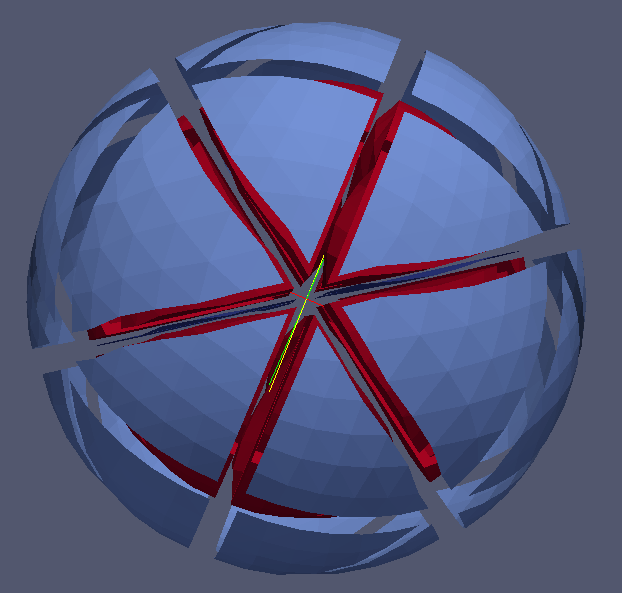
\includegraphics[scale=0.21]{images/32-full}  \captionsetup{width=0.6\textwidth} \caption{ Entities of all structural types visualised together } \end{subfigure}
	\caption{Presented is the 32 tetrahedron mesh loaded on 2 cores, visualising the entities of the grid of various structural types. }
	\label{fig:result:spherestruct}
\end{figure}

\begin{figure}
    \centering
	\begin{subfigure}[b]{0.48\textwidth} 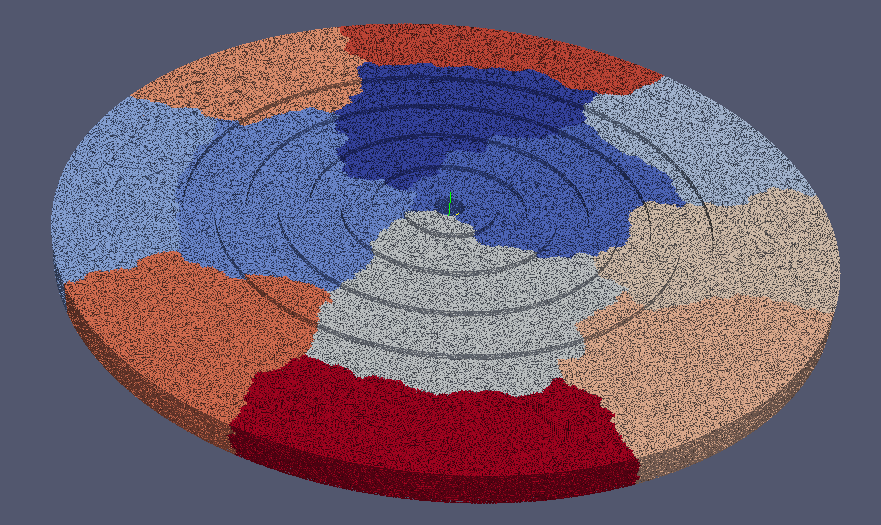
\includegraphics[scale=0.20]{images/bullseye-core-angle}          \captionsetup{width=0.8\textwidth} \caption{Interior elements coloured by owner process}   \end{subfigure}
	\begin{subfigure}[b]{0.48\textwidth} 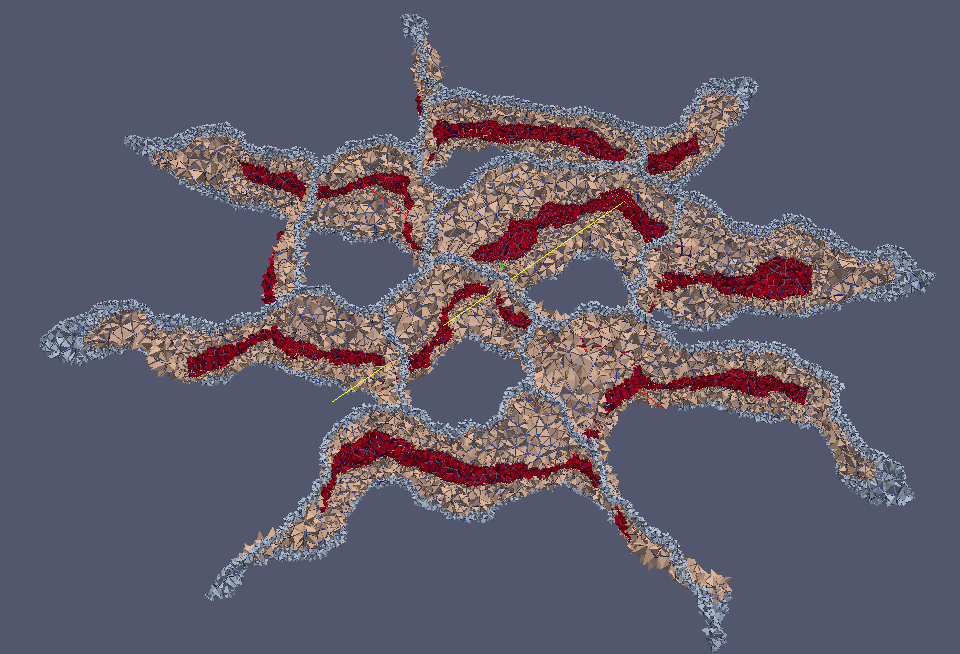
\includegraphics[scale=0.17]{images/bullseye-ghostelements-angle}  \captionsetup{width=0.8\textwidth} \caption{Ghost elements, coloured by material property} \end{subfigure}
	\caption{Presented is the 4.4 million tetrahedral mesh of Bulls Eye geometry.}
	\label{fig:result:bullseye}
\end{figure}

\noindent
Among other features of CurvGrid are: Global Index for all entities, Ghost Elements, DataHandle communication for entities of all codimensions, Nearest neighbour communication, Logging and Timing mechanisms, Curvilinear Grid diagnostics. A set of tutorial programs is provided to demonstrate the usage of various features of the grid. \\

\noindent
Below we list the functionality that is currently NOT available in the CurvGrid, but would be desirable to have. We welcome contributions from the community \\

\noindent
\begin{tabularx}{\textwidth}{l X}
\hline
     Difficulty & Description \\
\hline
	 Easy & Using GMSH partition tags to read pre-partitioned meshes \\
	 Medium & All-to-all communication paradigm to enable modelling of dense problems (e.g. Surface Integral Equation \cite{kern+2009}) \\
	 Medium & Curvilinear Grid optimization for parallel scalability using nearest neighbour communication \\
	 Medium & Curvilinear Meshes of non-uniform order \\
	 Medium & Utility to efficiently locate the element containing a given global coordinate (via OCTree) \\
	 Medium & Periodic and interior boundaries \\
	 Medium & 1D and 2D geometries \\
	 Medium & Does NOT support front/overlap elements at the moment \\
	 Hard & Non-tetrahedral geometries (e.g. Hexahedral) \\
	 Hard & Non-conformal meshes (Hanging nodes) \\
	 Hard & Global and Local Refinement \\
\hline
\end{tabularx}

%%%\subsection{Design decisions}
%%%\label{section-outline-designdecisions}
%%%
%%% Design decisions for Curvilinear Grid Factory
%%%\begin{itemize}
%%%	\item User must provide globalId's for vertices and elements. [Automatically implemented by GMSH \citeGMSH]
%%%	\item User must provide all boundary segments inside GMSH file.
%%%\end{itemize}


\subsection{Internal Structure}
\label{section-outline-internalstructure}

Below we present a simplified structure of classes used by Curvilinear Grid and geometry \\

\noindent
\begin{tabularx}{\textwidth}{ l | X }
\hline
   Class Name & Description \\ \hline
   CurvilinearGeometry                & Core class complying with dune-geometry standard \\ \hline
   * CurvilinearGeometryHelper        & Auxiliary functions, subentities for curvilinear elements \\ \hline
   * LagrangeInterpolator             & Lagrange Interpolation of element geometry \\ \hline
   * Polynomial                       & Analytic polynomial routines \\ \hline
   * DifferentialHelper               & Analytic Curvilinear Jacobians and Integration elements \\ \hline
   * IntegralHelper                   & Integral Functors, analytic integration routines  \\ \hline
   * QuadratureIntegrator             & Recursive integration using numerical quadrature. Performs fast \\ \hline
   * AdaptiveIntegrator               & Recursive integration using adaptive refinement. Performs slowly \\ \hline
  CurvilinearGMSHReader               & Reads a $.msh$ file and supplies entities to a Grid Factory \\ \hline
  * Gmsh2DuneMapper                   & Converts between interpolation vertex numbering paradigms \\ \hline
  CurvilinearVTKWriter                & Writes curvilinear elements to VTK, VTU/PVTU files \\ \hline
  CurvilinearVTKGridWriter            & Writes Curvilinear Grid to VTK, VTU/PVTU files \\ \hline
  CurvilinearGridBase                 & Lower level grid implementation. All entities are given by their codimension and index \\ \hline
  * CurvilinearGridStorage            & Storage class for entire grid \\ \hline
  * CurvilinearGridConstructor        & Constructs entities of the grid, finds neighbouring processes, generates global index \\ \hline
  * CurvilinearGhostConstructor       & Constructs ghost entities \\ \hline
  * CurvilinearPostConstructor        & Enables DataHandle communication \\ \hline
  Curvilinear Grid                    & Core class complying with dune-grid standard \\ \hline
  * CurvilinearGridFactory            & Interface for constructing Curvilinear Grid \\ \hline
  * CurvilinearGridDiagnostics        & Tests and collects statistics on Curvilinear Grid \\ \hline
  * LoggingMessage                    & Logging output with varying levels of verbosity \\ \hline
  * LoggingTimer                      & Parallel timing of parts of code. \\ \hline
  * AllCommunicate                    & Nearest neighbour communication for POD. Wrapper for $MPI\_alltoallv$ \\ \hline
  * VectorHelper                      & Manipulation of vectors (union, intersection, complement), as well as conversion to string \\ \hline
\end{tabularx}
